\section{Latihan}
Bisa karena biasa, rumit karena tak di cicil. Maka pemakaian git adalah maslaha kebiasaan. Oleh karena itu, dalam pembukaan awal buku ini justru kita tidak dulu masuk kepada teori git tapi langsung praktek. setelah berkali-kali praktek maka akan timbul beberapa pertanyaan mengenai fungsi dari perintah-perintah git yang bisa di baca pada bagian selanjutnya.

Skenarionya adalah, kita akan melakukan kontribusi terhadap sebuah repo Open Source di GitHub. Jadi latihan ini adalah latihan bagaimana ikut berkontribusi kepada repo Open Source yang ada di Github yang selama ini digunakan oleh para relawan kode untuk bersama membangun kode program berbasis Open Source.
\subsection{Konfigurasi Key}
Pertama kita masuk kepada tahapan seting atau konfigurasi key untuk mengakses semua repo dari profile kita dari git bash:
\begin{enumerate}
\item Buat Akun di Github.com Terlebih dahulu
\item install git bash di komputer anda, kemudian buka git bash.
\item Pastikan sudah ada di home direktori dengan mengetikkan perintah cd kemudian enter. Uktuk mengetahui posisi anda ada di direktori mana ketikkan perintah pwd dan enter.
\item Generate Key dengan perintah
\verb|ssh-keygen -t rsa -b 4096 -C "your_email@example.com"|
\item Baca key yang sudah di generate, gunakan perintah
\verb|cat .ssh/id_rsa.pub|
\item Hasil luaran yang dibaca sebelumnya merupakan key kita, masukkan key dengan masuk kepada menu Setting terus kepada menu SSH dan GPG Keys tambahkan New SSH key
\end{enumerate}

\subsection{Fork Repositori}
Pertama kita cari repositori utama yang akan kita ikut berkontribusi kepada repositori tersebut. Jika sudah ketemu, kemudian klik Fork(Tombol kanan atas) yang dilanjutkan dengan memilih akun kita sebagai tujuan clone fork tersebut. Setelah selesai maka kita akan memiliki repo yang sama dengan repo yang anda fork. Contoh apabila anda melakukan Fork dari https://github.com/RepoAsal/Testing maka anda akan memiliki repo https://github.com/usernameAnda/Testing, dan kita akan bekerja pada repo hasil fork ini.

\subsection{Navigasi direktori dengan Git Bash}
Pertama kita tentukan terlebih dahulu folder tempat kita mengerjakan repo hasil fork kita. Misal di Drive D: folder Ganteng. Maka buka git bash kita dan arahkan menuju folder tersebut dengan perintah \verb|cd /D/Ganteng| lalu buka web repo fork kita di github klik tombol hijau CLone or Download pilih Clone with SSH lalu salin kode yang tampak seperti git@github.com:usernameAnda/Testing.git. Pada Git Bash ketik git clone git@github.com:usernameAnda/Testing.git . Setelah selesai, ketik perintah ls maka akan muncul direktori baru yaitu folder Testing atau sesuai dengan nama repo anda. masuk ke direktori tersebut dengan perintah cd Testing. Kemudian ketik git status akan muncul status dari repo git kita.

\subsection{Sinkronisasi dengan Repo Utama}
Karena ini repo hasil Fork maka kita harus selalu di sinkronisasi dari repo aslinya(tidak otomatis tersingkron). Sehingga perlu melakukan setting sumber repo tujuan yang merupakan repo asal. Pertama pastikan git bash sudah pada direktori repositori. Untuk melakukan sinkronisasi dengan repo asal kita harus mengeset satu kali dengan perintah :
\verb|git remote add upstream https://github.com/RepoAsal/Testing.git|

Setelah melakukan setting sekali di awal, kemudian selanjutnya kita tinggal melakukan sinkronisasi terus menerus sebelum melakukan perubahan dengan dua perintah berikut :
\begin{verbatim}
git fetch upstream
git pull upstream master
\end{verbatim}


\subsection{Bekerja dengan Git Bash}
Sekarang kita mulai bekerja pada repo kita. Melakukan penambahan atau perubahan pada file. Kemudian perubahan tersebut diminta untuk dimasukkan di repo utama tempat kita fork repo kita. Urutan pekerjaan yang kita ulang terus menerus adalah sebagai berikut :
\begin{enumerate}
\item git fetch upstream
\item git pull upstream master
\item git push origin master
\item Silahkan edit satu file yang akan di ubah atau ditambah lalu di simpan dan di tutup yang berada di direktori yang sudah disetting di navigasi direktori.
    \begin{figure}[!htbp]
        \centering
            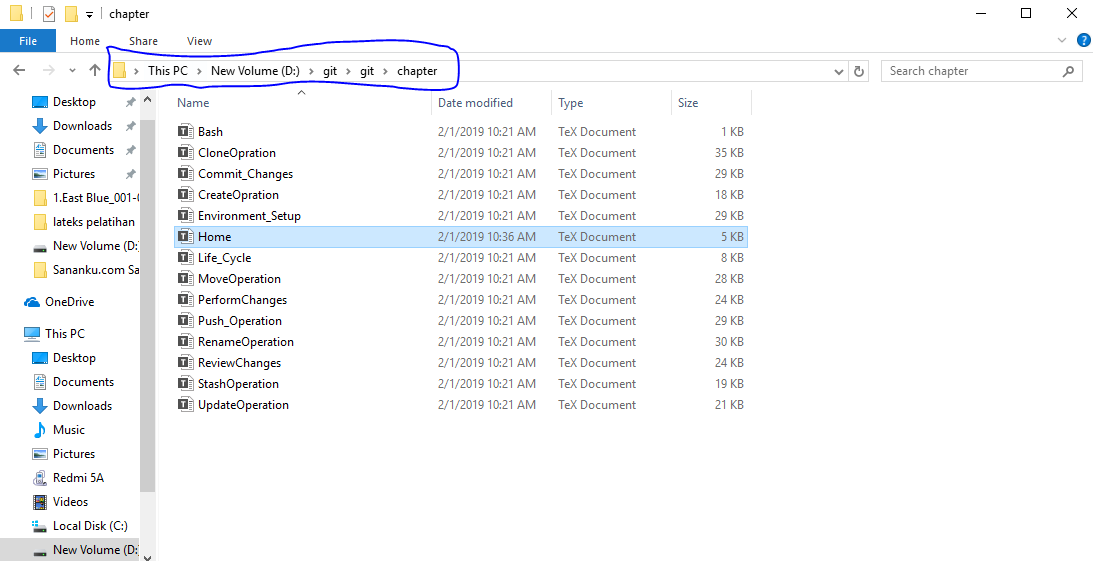
\includegraphics[width=3cm,height=3cm]{Capture}
            \caption{Direktori}
        \label{penanda}
    \end{figure}
\item git status
\item untuk memasukkan file yang sudah diubah/diedit yaitu dengan perintah `git add namafilenya.tex`
\item git status
\item git commit -m `perubahan apa yang telah kita lakukan di ceritakan di sini secara lengkap'
\item git status
\item git push origin master
\item buka web repo kita di github.com, contoh disini https://github.com/usernameAnda/Testing kemudian klik New pull request. Pastikan yang sebelah kiri atau base kita set kepada repo utama tempat fork kita yaitu RepoAsal/Testing dan compare pada sebelah kanan adalah repo kita, disini dicontohkan usernameAnda/Testing. Klik tombol hijau `Create Pull Request'. Share. Dan klik kembali tombol hijau lagi.
\item Beritahukan admin repo utama untuk accept Pull Request anda. Jika sudah di accept lakukan lagi langkah dari awal.
\end{enumerate} 